\chapter{Diseño}

    \chapter{Implementación del Sistema Backend Serverless}
    \label{ch:implementacion}

    \section{Introducción}
    El presente capítulo describe las etapas de implementación de la solución propuesta, basada en una arquitectura de microservicios sin servidor (\textbf{Serverless}). Se detalla la configuración de los componentes en la nube de Amazon Web Services (AWS) y el proceso de despliegue continuo utilizando el marco de trabajo \textbf{AWS Serverless Application Model (SAM)}.

    \section{Arquitectura Serverless}
    La solución se implementó bajo un modelo Serverless, minimizando la gestión de infraestructura y optimizando la escalabilidad y el costo. Los componentes principales se ilustran en la Figura \ref{fig:arquitectura}.

    \begin{figure}[H]
        \centering
        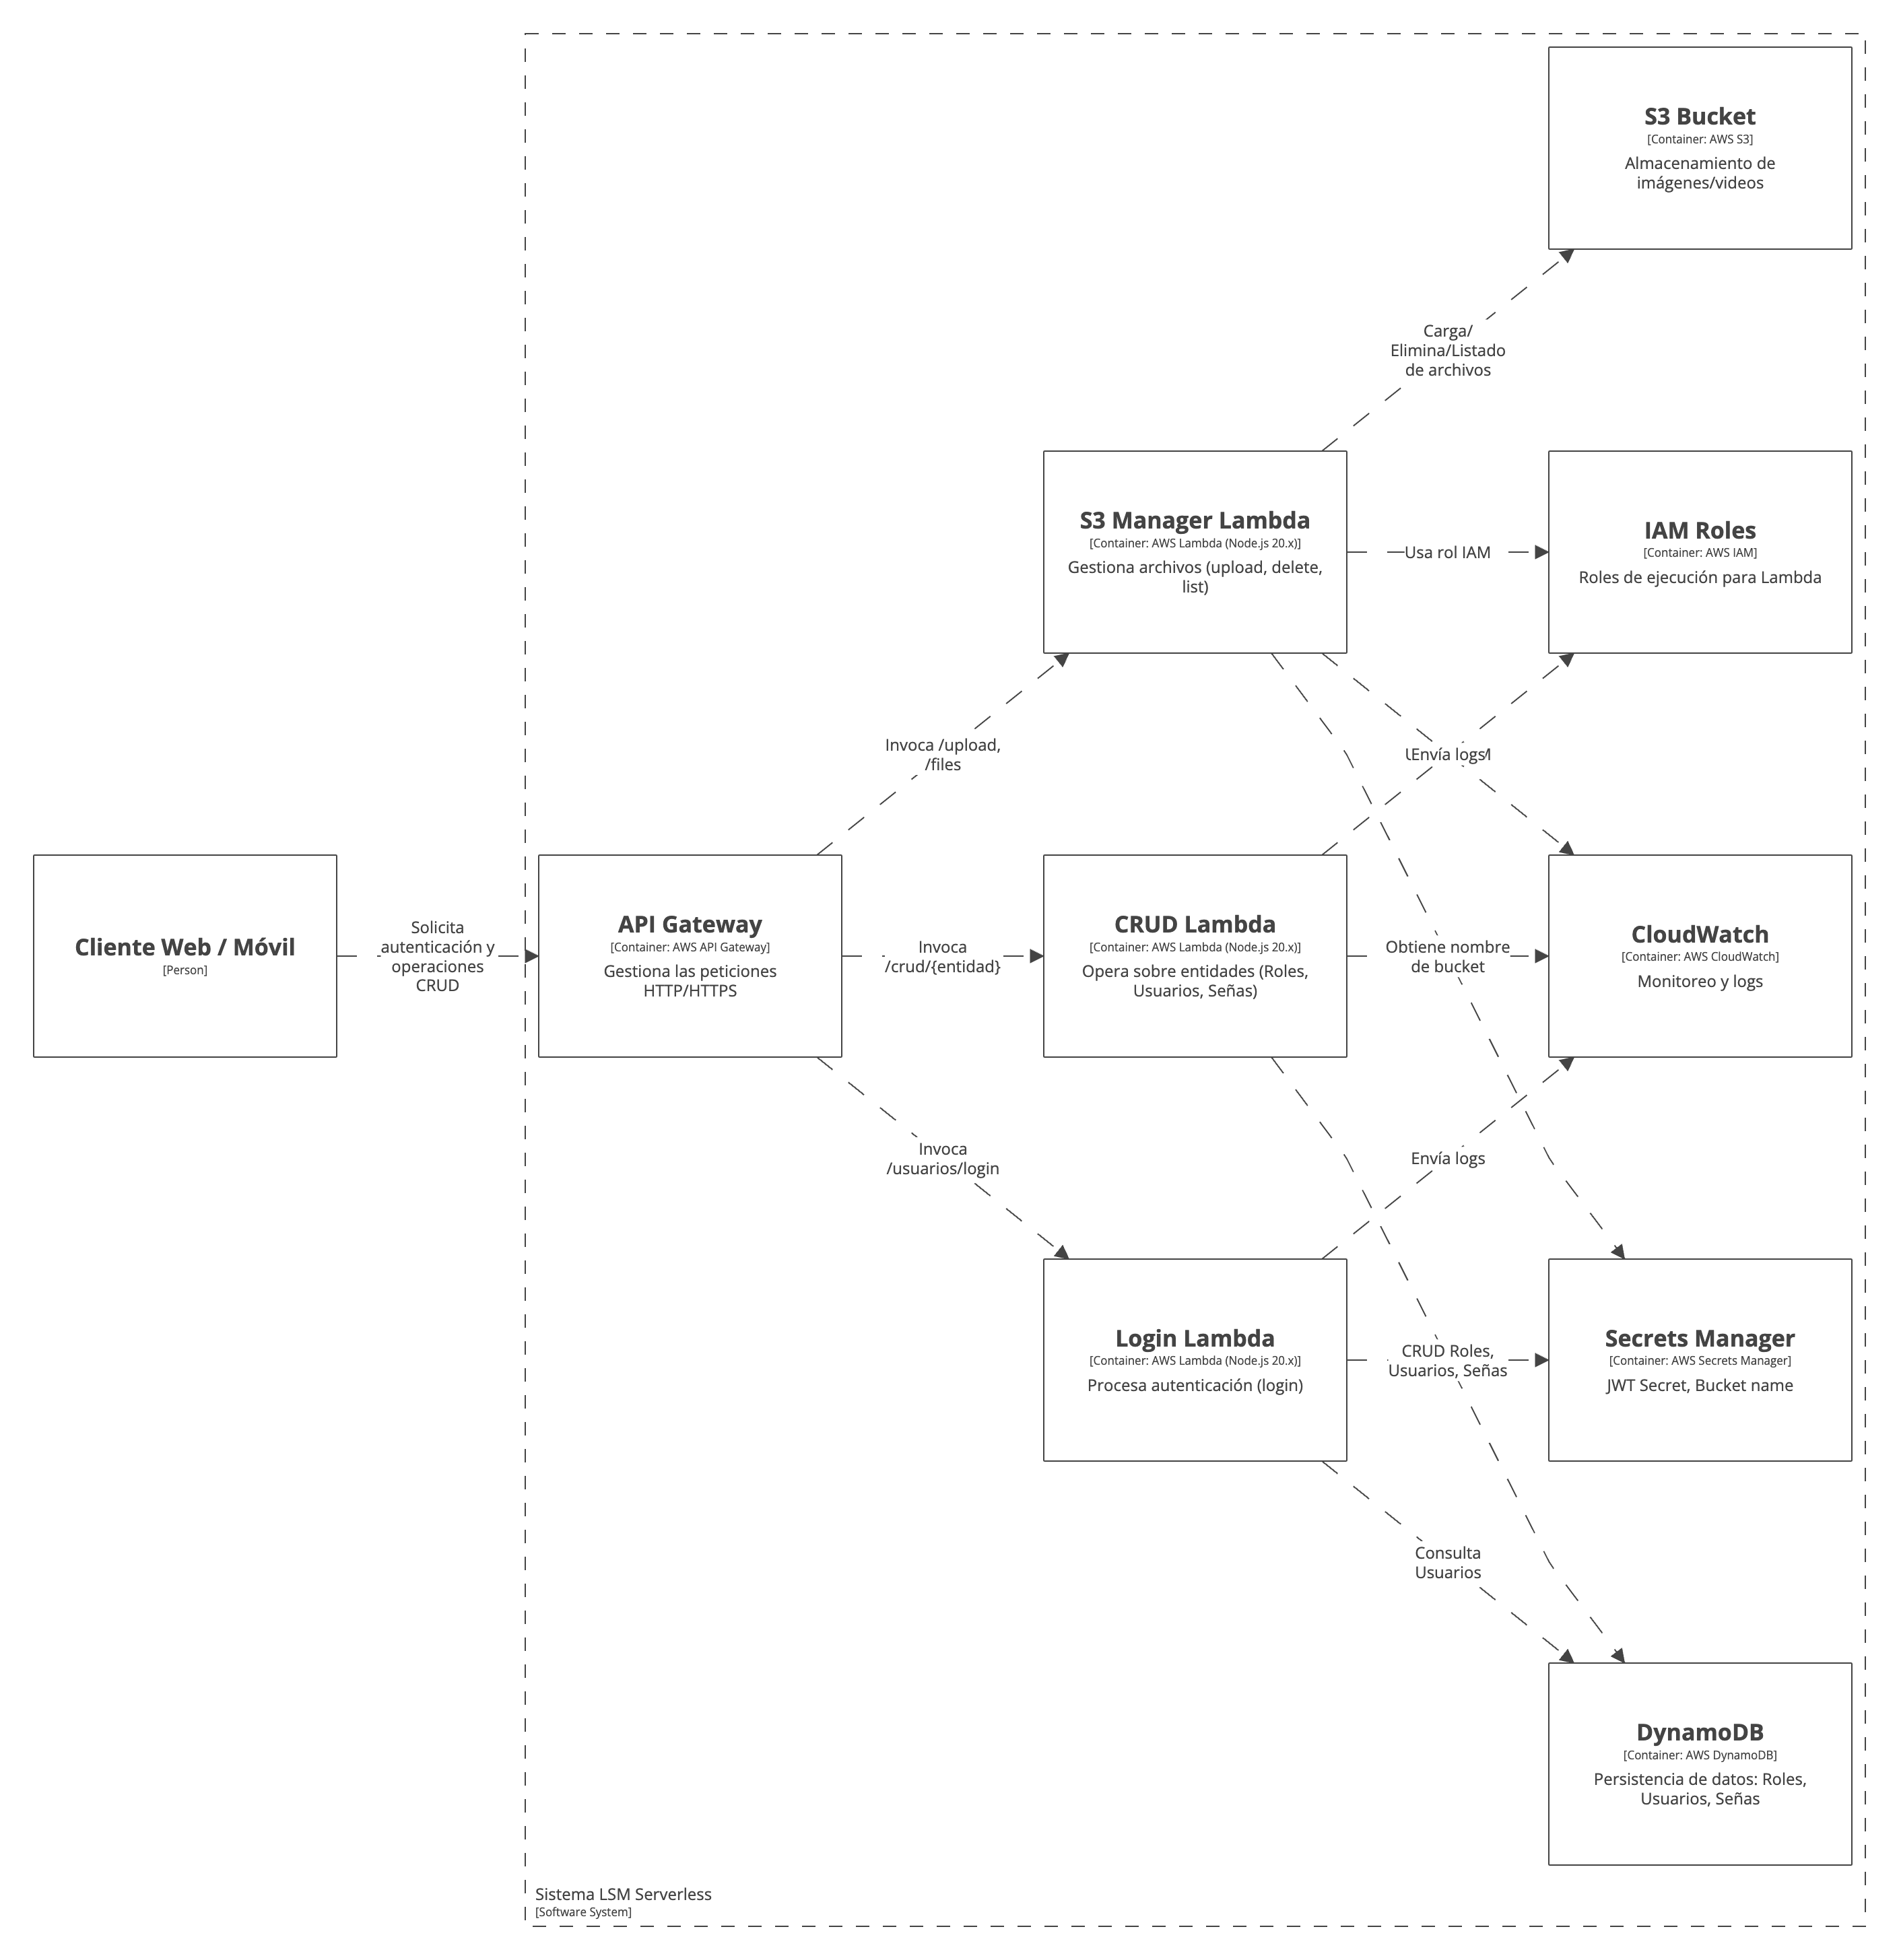
\includegraphics[width=0.8\textwidth]{CAPITULOS/capitulo6/diagrama.png} % Reemplaza con el nombre de tu diagrama
        \caption{Diagrama de Arquitectura Serverless de la Solución}
        \label{fig:arquitectura}
    \end{figure}

    La arquitectura se compone de tres servicios principales, cada uno gestionado por una función AWS Lambda dedicada:

    \begin{enumerate}
        \item \textbf{Servicio de Autenticación (\texttt{logginFunction})}: Maneja el inicio de sesión y la generación de tokens JWT.
        \item \textbf{Servicio CRUD (\texttt{CrudFunction})}: Gestiona las operaciones de alta, consulta, actualización y eliminación de datos en DynamoDB.
        \item \textbf{Servicio de Gestión de Archivos (\texttt{S3BucketManager})}: Administra la subida y eliminación de archivos en el bucket S3.
    \end{enumerate}

    \section{Implementación de Base de Datos}
    Los datos estructurados se almacenan en tres tablas de DynamoDB (\texttt{Roles}, \texttt{Usuarios}, \texttt{Senas}), utilizando el campo \texttt{\_id} como clave de partición. El modelo de facturación es \textbf{On-Demand} (\texttt{PAY\_PER\_REQUEST}) para optimizar costos de acuerdo a la carga real.

    \subsection{Creación de Tablas con AWS CLI}
    El proceso de creación de tablas se automatizó mediante \textbf{AWS CLI}, asegurando la consistencia en el esquema y la configuración de facturación para las tres entidades principales del sistema:

    \begin{lstlisting}[language=bash, caption={Creación de tabla DynamoDB: Roles}]
aws dynamodb create-table \
  --table-name Roles \
  --attribute-definitions AttributeName=_id,AttributeType=S \
  --key-schema AttributeName=_id,KeyType=HASH \
  --billing-mode PAY_PER_REQUEST
    \end{lstlisting}

    \begin{lstlisting}[language=bash, caption={Creación de tabla DynamoDB: Usuarios}]
aws dynamodb create-table \
  --table-name Usuarios \
  --attribute-definitions AttributeName=_id,AttributeType=S \
  --key-schema AttributeName=_id,KeyType=HASH \
  --billing-mode PAY_PER_REQUEST
    \end{lstlisting}

    \begin{lstlisting}[language=bash, caption={Creación de tabla DynamoDB: Senas}]
aws dynamodb create-table \
  --table-name Senas \
  --attribute-definitions AttributeName=_id,AttributeType=N \
  --key-schema AttributeName=_id,KeyType=HASH \
  --billing-mode PAY_PER_REQUEST
    \end{lstlisting}

    \subsection{Carga Inicial de Datos}
    Los datos iniciales para los roles, usuarios y el catálogo de señas fueron cargados utilizando operaciones de escritura por lotes (\texttt{batch-write-item} para el catálogo de señas) y elementos individuales (\texttt{put-item} para roles y usuarios iniciales) desde archivos de formato \texttt{JSON}.

    \subsection{Gestión de Identidad y Acceso (AWS IAM)}
    Para gestionar los accesos, se definió un rol de ejecución único \texttt{lambda-execution-role} con permisos centralizados para las funciones Lambda. Este rol incluye políticas específicas para interactuar con las tablas \textbf{Roles}, \textbf{Usuarios} y \textbf{Senas}, además de los permisos necesarios para la gestión del bucket S3, como se especifica en \texttt{roleLambda.yaml}.

    \begin{lstlisting}[language=yaml, caption={Fragmento del template para rol de ejecución Lambda (\texttt{roleLambda.yaml})}]
Policies:
  - PolicyName: lambda-custom-policy
    PolicyDocument:
      Version: "2012-10-17"
      Statement:
        - Effect: Allow
          Action:
            - dynamodb:GetItem
            - dynamodb:PutItem
            - dynamodb:UpdateItem
            - dynamodb:DeleteItem
            - dynamodb:Query
            - dynamodb:Scan
          Resource:
            - !Sub 'arn:aws:dynamodb:${AWS::Region}:${AWS::AccountId}:table/Roles'
            - !Sub 'arn:aws:dynamodb:${AWS::Region}:${AWS::AccountId}:table/Usuarios'
            - !Sub 'arn:aws:dynamodb:${AWS::Region}:${AWS::AccountId}:table/Senas'
        - Effect: Allow
          Action:
            - s3:PutObject
            - s3:GetObject
            - s3:DeleteObject
            - s3:ListBucket
          Resource:
            - !Sub 'arn:aws:s3:::${BucketName}/*'
            - !Sub 'arn:aws:s3:::${BucketName}'
    \end{lstlisting}

    \section{Despliegue y Funciones Lambda}
    El despliegue de funciones Lambda y API Gateways se realizó con \textbf{AWS SAM}. Cada función se implementó en un \texttt{Resource} separado para mantener la modularidad.

    \subsection{Función de Autenticación}
    \texttt{logginFunction} es el componente encargado de autenticar a los usuarios registrados en la base de datos y emitir un token JWT válido.

    \begin{lstlisting}[language=yaml, caption={Fragmento del template para logginFunction}]
Resources:
  LogginApiGateway:
    Type: AWS::Serverless::Api
    Properties:
      StageName: Prod
      Cors:
        AllowMethods: "'GET,POST,PUT,DELETE,OPTIONS'"
        AllowOrigin: "'*'"

  logginFunction:
    Type: AWS::Serverless::Function
    Properties:
      CodeUri: logging/
      Handler: app.handler
      Runtime: nodejs20.x
      Role: !Sub "arn:aws:iam::${AWS::AccountId}:role/lambda-execution-role"
      Events:
        LoginApi:
          Type: Api
          Properties:
            RestApiId: !Ref LogginApiGateway
            Path: /usuarios/login
            Method: post
    \end{lstlisting}

    \subsection{Función CRUD de Señas}
    \texttt{CrudFunction} encapsula la lógica de negocio para las operaciones del \textbf{CRUD} sobre la colección \textbf{Senas}.

    \begin{lstlisting}[language=yaml, caption={Fragmento del template para CrudFunction}]
CrudApiGateway:
  Type: AWS::Serverless::Api
  Properties:
    StageName: Prod
    Cors:
      AllowMethods: "'GET,POST,PUT,DELETE,OPTIONS'"
      AllowOrigin: "'*'"

CrudFunction:
  Type: AWS::Serverless::Function
  Properties:
    CodeUri: crud/
    Handler: app.handler
    Runtime: nodejs20.x
    Role: !Sub "arn:aws:iam::${AWS::AccountId}:role/lambda-execution-role"
    Events:
      CrudApi:
        Type: Api
        Properties:
          RestApiId: !Ref CrudApiGateway
          Path: /crud/senas
          Method: any
    \end{lstlisting}

    \subsection{Función de Gestión de Archivos S3}
    \texttt{S3BucketManager} se encarga de la interacción con el servicio \textbf{AWS S3}.

    \begin{lstlisting}[language=yaml, caption={Fragmento del template para S3BucketManager}]
S3ApiGateway:
  Type: AWS::Serverless::Api
  Properties:
    StageName: Prod
    Cors:
      AllowMethods: "'POST,DELETE,OPTIONS'"
      AllowOrigin: "'*'"

S3BucketManager:
  Type: AWS::Serverless::Function
  Properties:
    CodeUri: s3-manager/
    Handler: app.handler
    Runtime: nodejs20.x
    Role: !Sub "arn:aws:iam::${AWS::AccountId}:role/lambda-execution-role"
    Events:
      UploadApi:
        Type: Api
        Properties:
          RestApiId: !Ref S3ApiGateway
          Path: /upload
          Method: post
      DeleteApi:
        Type: Api
        Properties:
          RestApiId: !Ref S3ApiGateway
          Path: /files/{key+}
          Method: delete
    \end{lstlisting}

    \subsection{Resumen de Endpoints}

    \begin{table}[H]
        \centering
        \caption{Endpoints y Operaciones de la Función \texttt{logginFunction}}
        \renewcommand{\arraystretch}{1.3}
        \begin{tabularx}{\textwidth}{|p{4cm}|p{5cm}|X|}
            \hline
            \textbf{Función Lambda} & \textbf{Método HTTP / Ruta (Endpoint)} & \textbf{Descripción} \\ \hline
            \texttt{logginFunction} & POST \texttt{/usuarios/login} & \textbf{Autenticación de Usuarios.} Verifica credenciales (correo/contraseña) en la tabla \texttt{Usuarios} de DynamoDB y, si son válidas, emite un \textbf{Token JWT} para su uso en las demás APIs protegidas. \\ \hline
        \end{tabularx}
        \label{tab:logging_endpoints}
    \end{table}

    \begin{table}[H]
        \centering
        \caption{Endpoints y Operaciones de la Función \texttt{CrudFunction}}
        \renewcommand{\arraystretch}{1.3}
        \begin{tabularx}{\textwidth}{|p{4cm}|p{5cm}|X|}
            \hline
            \textbf{Función Lambda} & \textbf{Método HTTP / Ruta (Endpoint)} & \textbf{Descripción} \\ \hline
            \texttt{CrudFunction} & GET \texttt{/crud/senas} & \textbf{Consulta de Señas.} Recupera una o varias señas (mediante filtros o escaneo total) de la tabla \texttt{Senas}. \\ \hline
            \texttt{CrudFunction} & POST \texttt{/crud/senas} & \textbf{Creación de Seña.} Inserta un nuevo registro en la tabla \texttt{Senas} de DynamoDB. \\ \hline
            \texttt{CrudFunction} & PUT \texttt{/crud/senas} & \textbf{Actualización de Seña.} Modifica los campos de un registro de seña existente, identificado por su clave. \\ \hline
            \texttt{CrudFunction} & DELETE \texttt{/crud/senas} & \textbf{Eliminación de Seña.} Borra un registro de seña de la base de datos. \\ \hline
        \end{tabularx}
        \label{tab:crud_endpoints}
    \end{table}

    \begin{table}[H]
        \centering
        \caption{Endpoints y Operaciones de la Función \texttt{S3BucketManager}}
        \renewcommand{\arraystretch}{1.3}
        \begin{tabularx}{\textwidth}{|p{4cm}|p{5cm}|X|}
            \hline
            \textbf{Función Lambda} & \textbf{Método HTTP / Ruta (Endpoint)} & \textbf{Descripción} \\ \hline
            \texttt{S3BucketManager} & POST \texttt{/upload} & \textbf{Subida de Archivos.} Carga archivos (imágenes/videos) al bucket S3. Esta operación genera la URL de acceso que se almacena posteriormente en DynamoDB. \\ \hline
            \texttt{S3BucketManager} & DELETE \texttt{/files/\{key+\}} & \textbf{Eliminación de Archivos.} Borra un objeto específico (archivo) del bucket S3, utilizando la clave del archivo como parámetro de ruta. \\ \hline
        \end{tabularx}
        \label{tab:s3_endpoints}
    \end{table}

    \section{Proceso de Despliegue con SAM CLI}
    El flujo estándar para el despliegue de la aplicación Serverless incluye el uso de la interfaz de línea de comandos \textbf{SAM CLI}.

    \begin{enumerate}
        \item \textbf{Construcción:}
        \begin{lstlisting}[language=bash, caption={SAM Build}]
rm -rf .aws-sam/
sam build
        \end{lstlisting}

        \item \textbf{Despliegue:}
        \begin{lstlisting}[language=bash, caption={SAM Deploy}]
sam deploy
        \end{lstlisting}
    \end{enumerate}

    \section{Conclusión}
    La implementación en AWS con un enfoque Serverless resultó eficiente y escalable. El uso de \textbf{Infraestructura como Código (IaC)} con \textbf{AWS SAM} garantizó reproducibilidad y control de versiones.
